\documentclass[
	% -- opções da classe memoir --
	12pt,				% tamanho da fonte
	openany,			% capítulos começam em pág ímpar (insere página vazia caso preciso)
  oneside,      % para impressão em página única. Oposto ao twoside (Nunca habilitar os dois!)
	%twoside,			% para impressão em recto e verso. Oposto a oneside (Nunca habilitar os dois!)
	a4paper,			% tamanho do papel. 
	% -- opções da classe abntex2 --
	%chapter=TITLE,		% títulos de capítulos convertidos em letras maiúsculas
	%section=TITLE,		% títulos de seções convertidos em letras maiúsculas
	%subsection=TITLE,	% títulos de subseções convertidos em letras maiúsculas
	%subsubsection=TITLE,% títulos de subsubseções convertidos em letras maiúsculas
	% -- opções do pacote babel --
	english,			% idioma adicional para hifenização
	french,				% idioma adicional para hifenização
	spanish,			% idioma adicional para hifenização
	brazil				% o último idioma é o principal do documento
	]{abntex2}

% ---
% Pacotes básicos 
% ---
\usepackage{lmodern}			  % Usa a fonte Latin Modern			
\usepackage[T1]{fontenc}		% Selecao de codigos de fonte.
\usepackage[utf8]{inputenc} % Codificacao do documento (conversão automática dos acentos)
\usepackage{lastpage}			  % Usado pela Ficha catalográfica
\usepackage{indentfirst}    % Indenta o primeiro parágrafo de cada seção.
\usepackage{color}				  % Controle das cores
\usepackage{graphicx}			  % Inclusão de gráficos
\usepackage{subfig}         % Sub-figuras
\usepackage{microtype}      % para melhorias de justificação
\usepackage{textcomp}       % Adiciona símbolo de trademark e outros ao T1
\usepackage{array}          % Usado nas tabelas com \newline
\usepackage{multirow}       % Define tabelas multirow
\usepackage[outputdir=Gen]{minted}
\usepackage{listings}       % Program listings
\usepackage{lscape}         % 90-degree rotated images and tables
\usepackage{longtable}      % multiple pages tables
		
% ---
% Pacotes adicionais, usados apenas no âmbito do Modelo Canônico do abnteX2
% ---
\usepackage{lipsum}				% para geração de dummy text
% ---

% ---
% Pacotes de citações
% ---
\usepackage[brazilian,hyperpageref]{backref}	 % Paginas com as citações na bibl
\usepackage[alf]{abntex2cite}	% Citações padrão ABNT

% Copiado das configurações do LyX

%%%%%%%%%%%%%%%%%%%%%%%%%%%%%% LyX specific LaTeX commands.
%% Because html converters don't know tabularnewline
\providecommand{\tabularnewline}{\\}

%%%%%%%%%%%%%%%%%%%%%%%%%%%%%% User specified LaTeX commands.

% --- 
% CONFIGURAÇÕES DE PACOTES
% --- 

% ---
% Configurações do pacote backref
% Usado sem a opção hyperpageref de backref
\renewcommand{\backrefpagesname}{Citado na(s) página(s):~}
% Texto padrão antes do número das páginas
\renewcommand{\backref}{}
% Define os textos da citação
\renewcommand*{\backrefalt}[4]{
	\ifcase #1 %
		Nenhuma citação no texto.%
	\or
		Citado na página #2.%
	\else
		Citado #1 vezes nas páginas #2.%
	\fi}%
% ---

% --- 
% NOME DA BASE
% --- 

% ---
% Nome da base
\newcommand{\databaseName}{Sorveteria}
\newcommand{\storeName}{Gelatto Felice}
\newcommand{\storeFullName}{Sorveteria \storeName{}}
% ---


% ---
% Informações de dados para CAPA e FOLHA DE ROSTO
% ---
\titulo{Planejamento ETL da Base de Dados de uma Sorveteria}
\autor{André Ferreira Bem Silva\\ Augusto Gonçalves\\Fernando D'Império\\Marcos Vinício de Siqueira}

\local{São Paulo, SP}
\data{25/02/2017}
\instituicao{%
  Fundação Getúlio Vargas -- FGV
  \par
  MBA Executivo em Economia e Gestão: Business Analytics e Big Data T3
  \par
  Disciplina de Análise Exploratória de Dados
}
\tipotrabalho{Relatório}
% O preambulo deve conter o tipo do trabalho, o objetivo, 
% o nome da instituição e a área de concentração 
\preambulo{Este trabalho contém uma análise sobre o modelo de dados da rede \emph{\storeFullName} para que seja possível extrair-se um modelo \emph{snowflake} com relação as vendas dessa rede de lojas.}
% ---


% ---
% Configurações de aparência do PDF final

% alterando o aspecto da cor azul
\definecolor{blue}{RGB}{41,5,195}

% informações do PDF
\makeatletter
\hypersetup{
     	%pagebackref=true,
		pdftitle={\@title}, 
		pdfauthor={\@author},
    	pdfsubject={\imprimirpreambulo},
	    pdfcreator={LaTeX with abnTeX2},
		pdfkeywords={abnt}{latex}{abntex}{abntex2}{trabalho acadêmico}, 
		colorlinks=true,       		% false: boxed links; true: colored links
    	linkcolor=blue,          	% color of internal links
    	citecolor=blue,        		% color of links to bibliography
    	filecolor=magenta,      		% color of file links
		urlcolor=blue,
		bookmarksdepth=4
}
\makeatother
% --- 

% --- 
% Espaçamentos entre linhas e parágrafos 
% --- 

% O tamanho do parágrafo é dado por:
\setlength{\parindent}{1.3cm}

% Controle do espaçamento entre um parágrafo e outro:
\setlength{\parskip}{0.2cm}  % tente também \onelineskip

% ---
% compila o indice
% ---
\makeindex
% ---

% ----
% Início do documento
% ----
\begin{document}

% Seleciona o idioma do documento (conforme pacotes do babel)
%\selectlanguage{english}
\selectlanguage{brazil}

% Retira espaço extra obsoleto entre as frases.
\frenchspacing 

% ----------------------------------------------------------
% ELEMENTOS PRÉ-TEXTUAIS
% ----------------------------------------------------------
% \pretextual

% ---
% Capa
% ---
\imprimircapa
% ---

% ---
% Folha de rosto
% (o * indica que haverá a ficha bibliográfica)
% ---
\imprimirfolhaderosto
% ---

% ---

% ---

% ---

% ---
% inserir lista de ilustrações
% ---
%\pdfbookmark[0]{\listfigurename}{lof}
\listoffigures*
%\cleardoublepage
% ---

% ---
% inserir lista de tabelas
% ---
\pdfbookmark[0]{\listtablename}{lot}
%\listoftables*
\cleardoublepage
% ---

% ---
% inserir lista de abreviaturas e siglas
% ---
%\begin{siglas}
%  \item[ABNT] Associação Brasileira de Normas Técnicas
%  \item[abnTeX] ABsurdas Normas para TeX
%\end{siglas}
% ---

% ---
% inserir lista de símbolos
% ---
%\begin{simbolos}
%  \item[$ \Gamma $] Letra grega Gama
%  \item[$ \Lambda $] Lambda
%  \item[$ \zeta $] Letra grega minúscula zeta
%  \item[$ \in $] Pertence
%\end{simbolos}
% ---

% ---
% inserir o sumario
% ---
\pdfbookmark[0]{\contentsname}{toc}
\tableofcontents*
\cleardoublepage
% ---



% ----------------------------------------------------------
% ELEMENTOS TEXTUAIS
% ----------------------------------------------------------
\textual

% ----------------------------------------------------------
% Introdução (exemplo de capítulo sem numeração, mas presente no Sumário)
% ----------------------------------------------------------
%\chapter*[Introdução]{Introdução}
%\addcontentsline{toc}{chapter}{Introdução}
% ----------------------------------------------------------

\graphicspath{{./Gen/Image/}{../Gen/Image/}{./Image/}}

%Adiciona introdução com numeração
\chapter[Introdução]{Introdução}
\section{Objetivo}

%Somos o banco X e vamos decidir se emprestamos ou não para o cliente Y (no nosso caso para a Positivo Informática S/A)
Por meio de uma análise detalhada e consolidada dos indicadores da empresa \nomeCompletoPositivo{}, define-se o risco de investimento na mencionada empresa por parte do \emph{\nomeDoBanco{}}. Sendo assim, essa análise deve definir, seguindo métricas e métodos de controladoria gerencial, uma recomendação ao \emph{board} do banco para que possam tomar uma decisão referente ao mesmo.

\section{Risco de Crédito}

\section{Histórico}
A Positivo Tecnologia nasceu do Grupo Positivo, que é o maior grupo do segmento de educação no Brasil. Fundado em 1972, a partir da criação de uma escola e de uma gráfica, o Grupo Positivo possui atualmente empresas líderes nos três segmentos em que atua: educacional, gráfico-editorial e tecnologia. A partir do grande sucesso de sua inovadora metodologia de ensino desenvolvida, aprimorada e sistematizada pelos conceituados professores fundadores do grupo, a rede de escolas próprias foi ampliada para os demais níveis educacionais e, em 1979, o grupo iniciou a venda de livros e serviços a outras escolas em todo Brasil.

Em 1989, os mesmos empreendedores do grupo iniciaram a produção de computadores pessoais, criando assim a Positivo Informática. Inicialmente, este ramo do grupo focou apenas na produção e comercialização de computadores para escolas clientes do Grupo Positivo em todo o Brasil. Atualmente, no ramo de tecnologia, a empresa produz computadores, laptops, tablets, smartphones, celulares e, mais recentemente, dispositivos de telemedicina. 

A semente original do grupo ainda se mantém, o grupo conta com cerca de 27 mil alunos em suas unidades próprias (Escolas Positivo, Curso Positivo e Universidade Positivo), além de ter atendido a aproximadamente 10 milhões de alunos com seus produtos e serviços desde sua fundação. Os Portais Educacionais do Grupo Positivo estão presentes em cerca de 11,0 mil escolas. Além disso, a Posigraf é a primeira gráfica Carbono Zero do país. O Grupo Positivo conta atualmente com mais de 9,0 mil colaboradores.

\section{Perfil Corporativo}

\begin{figure}[h]
\begin{centering}
\includegraphics[width=1.0\textwidth]{Img/Corporativo}
\caption{Figura que demonstra o domínio e capital social da \nomeCompletoPositivo{}.}
\par\end{centering}
\end{figure}

Em 2016, a Positivo Tecnologia foi uma das maiores fabricantes de computadores no Brasil, respondendo por 15,3\% do número total de computadores vendidos no mercado brasileiro, de acordo com a IDC. No mesmo período, obtiveram uma participação de 19,9\% do mercado de varejo. Uma parcela substancial da produção de computadores é vendida através de grandes redes de varejo, com as quais o grupo mantém sólido relacionamento comercial, em função principalmente dos preços competitivos, do reconhecimento da marca e assistência técnica.

Adicionalmente, a companhia atua no mercado argentino por meio da marca \nomePositivoAr{}, fruto de uma joint venture com um parceiro local. Em 2015, os computadores \nomePositivoAr{} atingiram uma participação de 9,5\%, segundo a IDC.

No Brasil, a Positivo Tecnologia oferece uma linha completa de dispositivos, incluindo computadores de mesa (desktops e all-in-ones), computadores portáteis (notebooks e netbooks) e tablets, que são produzidos em Manaus (AM). Em 2012, a Companhia ingressou no mercado de telefones celulares, com a oferta de smartphones e messaging phones.

\begin{figure}[h]
\begin{centering}
\includegraphics[width=1.0\textwidth]{Img/PositivoMundo}
\caption{Operações da \nomePositivo{} a nível mundial, bastante expressiva na América Latina e observa-se também sítios na África.}
\par\end{centering}
\end{figure}

Além disso, para atendimento e suporte aos milhões de consumidores finais, empresas e órgãos do governo, conta com uma ampla e capacitada rede de assistências técnicas cobrindo a totalidade do território nacional, e com a CRP - Central de Relacionamento Positivo, que registrou em média, 2,9 mil contatos diários em 2016. Grande parte destes contatos se refere a questões básicas sobre uso do computador, sistema operacional ou problemas com conexões, uma vez que muitos dos clientes estão adquirindo seu computador pela primeira vez.

Parcela menor da receita da Companhia provém do Segmento de Tecnologia Educacional, no qual acredita ser líder absoluto no País. A Companhia oferece soluções de infraestrutura e gestão, aplicativos e plataformas educacionais, portais de educação, além de formação de professores e acompanhamento pedagógico. Os portais têm mais de 1,2 milhões de usuários ativos, com modelo de receita recorrente mensal. 

As soluções educacionais da Positivo Tecnologia estão presentes em mais de 14 mil escolas e são exportadas para mais de 40 países. Dentre os principais produtos estão mesas educacionais, dispositivos móveis, lousas interativas, dispositivos de armazenamento e recarga, projetores, acess point, e sistema de gerenciamento de aulas. A Companhia é também distribuidor exclusivo no Brasil de empresas líderes no desenvolvimento e distribuição de software educacional, bem como distribui produtos da LEGO\texttrademark Education no território nacional.

Em 2016, a Companhia ingressou no mercado de tecnologia médica por meio da aquisição de 50\% do capital social da Hi Technologies S.A., empresa com forte foco em P\&D para a oferta de produtos inovadores em saúde.


\chapter{Modelo Relacional}
\label{chap:RelationalModel}Neste capítulo, é feito uma análise detalhada com relação a base
relacional utilizada no modelo da \emph{\databaseName{}} e as regras de negócios envolvidas. 

Num primeiro momento, é descrito o cenário de negócios da sorveteria e num segundo explica-se o modelo
relacional vigente, suas entidades e as relações entre elas.

\section{Regras de Negócio}
\label{section:BusinessRules}
Nesta seção é  discutida as principais regras de negócio de interesse e o cenário das mesmas.

A rede de sorveteria \storeName{} é uma rede multinacional e possui 35 lojas em 8 países. São eles: Brasil, Alemanha, França, Argentina, Estados Unidos, México, Uruguai e Paraguai. As lojas possuem administrações distintas e matriz única no Brasil.

Numa compra nesta \emph{loja}, o \emph{cliente} dirige-se até uma das unidades rede, escolhe o \emph{produto}, dado seu \emph{sabor}, o tipo de \emph{embalagem} e procede até o caixa, onde cada compra efetuada por um cliente deve gerar uma nota fiscal. Essa compra deve conter pelo menos uma unidade de sorvete. 

Sazonalmente, a franquia promove campanhas publicitárias e de códigos de \emph{cupons de desconto} e outras \emph{promoções} afim de aumentar o movimento, quantidade de vendas e a lucratividade geral das lojas franquiadas.

\section{Modelo relacional}

O modelo relacional, da figura \ref{figure:RelationalModel}, inclui as entidades \emph{Loja, Produto, Embalagem, Cliente}, presentes no cenário de negócio da seção \ref{section:BusinessRules}. Nesta seção analisa-se essas e outras entidades do modelo.

% A small example on how to use the "rotating" package.
%  Displays a figure and it's caption in landscape
\begin{landscape}
\begin{figure}[ht]
\begin{centering}
    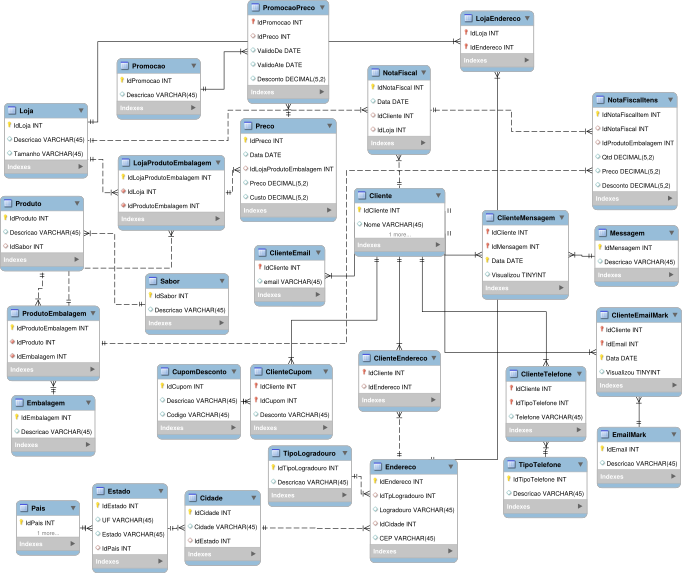
\includegraphics[width=1\textwidth]{RelationalModel}
    \caption{Modelo de base de dados relacional para a \storeFullName{}.}
    \label{figure:RelationalModel}
\end{centering}
\end{figure}
\end{landscape}

\section {Entidades}

Nesta seção, divide-se as entidades em \emph{fortes, fracas e associativas}. O objetivo dessa divisão é começar-se a entender quais são candidatas a serem chaves no modelo dimensional a ser utilizado.

\subsection{Entidades Fortes}
São as entidades que possuem chaves primárias independentes, e seus atributos podem ser unicamente identificados por ela. No modelo relacional da figura \ref{figure:RelationalModel}, são entidades fortes:

\begin{itemize}
\item \emph{Loja}: Define uma unidade da \storeFullName{}.
\item \emph{Produto}: Um produto da sorveteria. Ex: sorvete de chocolate.
\item \emph{Embalagem}: A embalagem de venda, com tamanho específico.
\item \emph{Cliente}: Informações a respeito do cliente da loja.
\end{itemize}

\subsection{Entidades Fracas}

É uma entidade cujos atributos não podem ser unicamente identificados sozinhos, portanto precisa de uma chave estrangeira ao menos para que isso aconteça. 

\begin{itemize}
\item \emph{Promocao}: Uma promoção sazonal da franquia.
\item \emph{CupomDesconto}: Um cupom de desconto específico.
\item \emph{TipoTelefone}: Telefone com DDD.
\item \emph{Sabor}: Um sabor de de sorvete.
\item \emph{EmailMark}: Endereço de e-mail.
\item \emph{Mensagem}: Uma mensagem enviada a um e-mail.
\item \emph{Endereco}: Endereço único (localidade).
\item \emph{TipoLogradouro}: Identifica o tipo de logradouro.
\item \emph{Cidade}: Identificação da cidade.
\item \emph{Estado}: Identificação do estado.
\item \emph{Pais}: Identificação do país.
\end{itemize}

\subsection{Entidades Associativas}

Uma entidade associativa é um termo de modelagem relacional que significa uma relação de muitos para muitos a nível de entidades e relações. As tabelas desse tipo são denominadas \emph{associativas}.

\begin{itemize}
\item \emph{ProdutoEmbalagem}: Relação entre Produto e Embalagem.
\item \emph{LojaProdutoEmbalagem}: Relação entre Loja e Produto com Embalagem.
\item \emph{Preco}: Associa um valor em moeda \emph{fiduciária} a um produto em determinado instante. Ex: Real, Dólar...
\item \emph{NotaFiscal}: Relatório de venda de produto(s).
\item \emph{NotaFiscalItens}: O relatório de um item de venda.
\item \emph{PromocaoPreco}: Preço referente a uma promoção específica.
\item \emph{ClienteCupom}: Cupom de um cliente.
\item \emph{ClienteEmail}: E-mail de um cliente.
\item \emph{ClienteEndereco}: Endereço de um  cliente.
\item \emph{ClienteTelefone}: Telefone de um cliente.
\item \emph{LojaEndereco}: Endereço de uma loja.
\item \emph{ClienteEmailMark}: Visualização de um determinado e-mail por parte do cliente.
\item \emph{ClienteMensagem}: Mensagem enviada ao cliente por e-mail.
\end{itemize}

\section{Dores do Negócio}
\label{section:BusinessPains}
O objetivo da modelagem dimensional a ser feita é responder os seguintes questionamentos:

\begin{enumerate}
\item Questões de Negócio/Analíticas
\item Quais são as lojas mais lucrativas?
\item Quais são os clientes que mais compram?
\item Quais promoções surtiram mais efeito?
\item Quais produtos mais vendem?
\end{enumerate}

Por isso, o modelo dimensional deverá ter como \emph{fato} principal a tabela \emph{Vendas}.


\chapter{Modelo Dimensional}
\label{chap:DimensionalModel} 

A modelagem dimensional (\emph{snowflake}) é feita a partir de uma tabela fato (Vendas) e suas dimensões. Na análise de dores de negócio no capítulo \ref{chap:RelationalModel}, seção \ref{section:BusinessRules}.

\section{Modelo Dimensional}

Na figura \ref{figure:RelationalModel}, observa-se o modelo dimensional de Vendas, com a tabela Fato no centro e as dimensões ao redor. A tabela a seguir é contém o plano de ETL modelo relacional para o modelo dimensional, com o qual obtém-se o modelo descrito na figura \ref{figure:RelationalModel}:

\begin{center}
\begin{figure}[ht]
\begin{centering}
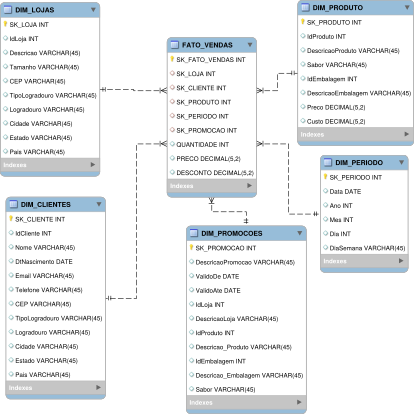
\includegraphics[width=0.8\textwidth]{DimensionalModel}
\par\end{centering}
  \caption{\label{figure:DimensionalModel}O modelo dimensional gerado a partir do modelo relacional, da figura \ref{figure:RelationalModel}, a ser carregado via ETL para um \emph{Data Warehouse/Mart}.}
\end{figure}
\vspace*{-40pt}
\par\end{center}


\begin{landscape}
\begin{longtable}{l|l|l|l|l|l|l|l|l}
\hline 
{\scriptsize{}Tabela} & {\scriptsize{}Coluna} & {\scriptsize{}Tipo Dado} & {\scriptsize{}Tipo} & {\scriptsize{}SCD} & {\scriptsize{}Tabela} & {\scriptsize{}Coluna} & {\scriptsize{}Tipo de Dado} & {\scriptsize{}Transformação}\tabularnewline
\hline 
{\scriptsize{}LOJAS} & {\scriptsize{}SK\_LOJA} & {\scriptsize{}INT} & {\scriptsize{}Dim} & {\scriptsize{}1} &  &  &  & {\scriptsize{}Surrogate Key}\tabularnewline
{\scriptsize{}LOJAS} & {\scriptsize{}IdLoja} & {\scriptsize{}INT} & {\scriptsize{}Dim} & {\scriptsize{}1} & {\scriptsize{}Loja} & {\scriptsize{}IdLoja} & {\scriptsize{}INT} & \tabularnewline
{\scriptsize{}LOJAS} & {\scriptsize{}Descricao} & {\scriptsize{}VARCHAR(45)} & {\scriptsize{}Dim} & {\scriptsize{}1} & {\scriptsize{}Loja} & {\scriptsize{}Descricao} & {\scriptsize{}VARCHAR(45)} & \tabularnewline
{\scriptsize{}LOJAS} & {\scriptsize{}Tamanho} & {\scriptsize{}VARCHAR(45)} & {\scriptsize{}Dim} & {\scriptsize{}1} & {\scriptsize{}Loja} & {\scriptsize{}Tamanho} & {\scriptsize{}VARCHAR(45)} & \tabularnewline
{\scriptsize{}LOJAS} & {\scriptsize{}CEP} & {\scriptsize{}VARCHAR(45)} & {\scriptsize{}Dim} & {\scriptsize{}1} & {\scriptsize{}Endereco} & {\scriptsize{}CEP} & {\scriptsize{}VARCHAR(45)} & \tabularnewline
{\scriptsize{}LOJAS} & {\scriptsize{}TipoLogradouro} & {\scriptsize{}VARCHAR(45)} & {\scriptsize{}Dim} & {\scriptsize{}1} & {\scriptsize{}TipoLogradouro} & {\scriptsize{}Descricao} & {\scriptsize{}VARCHAR(45)} & \tabularnewline
{\scriptsize{}LOJAS} & {\scriptsize{}Logradouro} & {\scriptsize{}VARCHAR(45)} & {\scriptsize{}Dim} & {\scriptsize{}1} & {\scriptsize{}Endereco} & {\scriptsize{}Logradouro} & {\scriptsize{}VARCHAR(45)} & \tabularnewline
{\scriptsize{}LOJAS} & {\scriptsize{}Cidade} & {\scriptsize{}VARCHAR(45)} & {\scriptsize{}Dim} & {\scriptsize{}1} & {\scriptsize{}Cidade} & {\scriptsize{}Cidade} & {\scriptsize{}VARCHAR(45)} & \tabularnewline
{\scriptsize{}LOJAS} & {\scriptsize{}Estado} & {\scriptsize{}VARCHAR(45)} & {\scriptsize{}Dim} & {\scriptsize{}1} & {\scriptsize{}Estado} & {\scriptsize{}Estado} & {\scriptsize{}VARCHAR(45)} & \tabularnewline
{\scriptsize{}LOJAS} & {\scriptsize{}Pais} & {\scriptsize{}VARCHAR(45)} & {\scriptsize{}Dim} & {\scriptsize{}1} & {\scriptsize{}Pais} & {\scriptsize{}Pais} & {\scriptsize{}VARCHAR(45)} & \tabularnewline
{\scriptsize{}CLIENTES} & {\scriptsize{}SK\_CLIENTE} & {\scriptsize{}INT} & {\scriptsize{}Dim} & {\scriptsize{}1} &  &  &  & {\scriptsize{}Surrogate Key}\tabularnewline
{\scriptsize{}CLIENTES} & {\scriptsize{}IdCliente} & {\scriptsize{}INT} & {\scriptsize{}Dim} & {\scriptsize{}1} & {\scriptsize{}Cliente} & {\scriptsize{}IdCliente} & {\scriptsize{}INT} & \tabularnewline
{\scriptsize{}CLIENTES} & {\scriptsize{}Nome} & {\scriptsize{}VARCHAR(45)} & {\scriptsize{}Dim} & {\scriptsize{}1} & {\scriptsize{}Cliente} & {\scriptsize{}Nome} & {\scriptsize{}VARCHAR(45)} & \tabularnewline
{\scriptsize{}CLIENTES} & {\scriptsize{}DtNascimento} & {\scriptsize{}DATE} & {\scriptsize{}Dim} & {\scriptsize{}1} & {\scriptsize{}Cliente} & {\scriptsize{}DtNascimento} & {\scriptsize{}DATE} & \tabularnewline
{\scriptsize{}CLIENTES} & {\scriptsize{}Email} & {\scriptsize{}VARCHAR(45)} & {\scriptsize{}Dim} & {\scriptsize{}1} & {\scriptsize{}ClienteEmail} & {\scriptsize{}Email} & {\scriptsize{}VARCHAR(45)} & \tabularnewline
{\scriptsize{}CLIENTES} & {\scriptsize{}Telefone} & {\scriptsize{}VARCHAR(45)} & {\scriptsize{}Dim} & {\scriptsize{}1} & {\scriptsize{}ClienteTelefone} & {\scriptsize{}Telefone} & {\scriptsize{}VARCHAR(45)} & \tabularnewline
{\scriptsize{}CLIENTES} & {\scriptsize{}CEP} & {\scriptsize{}VARCHAR(45)} & {\scriptsize{}Dim} & {\scriptsize{}1} & {\scriptsize{}Endereco} & {\scriptsize{}CEP} & {\scriptsize{}VARCHAR(45)} & \tabularnewline
{\scriptsize{}CLIENTES} & {\scriptsize{}TipoLogradouro} & {\scriptsize{}VARCHAR(45)} & {\scriptsize{}Dim} & {\scriptsize{}1} & {\scriptsize{}TipoLogradouro} & {\scriptsize{}Descricao} & {\scriptsize{}VARCHAR(45)} & \tabularnewline
{\scriptsize{}CLIENTES} & {\scriptsize{}Logradouro} & {\scriptsize{}VARCHAR(45)} & {\scriptsize{}Dim} & {\scriptsize{}1} & {\scriptsize{}Endereco} & {\scriptsize{}Logradouro} & {\scriptsize{}VARCHAR(45)} & \tabularnewline
{\scriptsize{}CLIENTES} & {\scriptsize{}Cidade} & {\scriptsize{}VARCHAR(45)} & {\scriptsize{}Dim} & {\scriptsize{}1} & {\scriptsize{}Cidade} & {\scriptsize{}Cidade} & {\scriptsize{}VARCHAR(45)} & \tabularnewline
{\scriptsize{}CLIENTES} & {\scriptsize{}Estado} & {\scriptsize{}VARCHAR(45)} & {\scriptsize{}Dim} & {\scriptsize{}1} & {\scriptsize{}Estado} & {\scriptsize{}Estado} & {\scriptsize{}VARCHAR(45)} & \tabularnewline
{\scriptsize{}CLIENTES} & {\scriptsize{}Pais} & {\scriptsize{}VARCHAR(45)} & {\scriptsize{}Dim} & {\scriptsize{}1} & {\scriptsize{}Pais} & {\scriptsize{}Pais} & {\scriptsize{}VARCHAR(45)} & \tabularnewline
{\scriptsize{}PRODUTOS} & {\scriptsize{}SK\_PRODUTO} & {\scriptsize{}INT} & {\scriptsize{}Dim} & {\scriptsize{}1} &  &  &  & {\scriptsize{}Surrogate Key}\tabularnewline
{\scriptsize{}PRODUTOS} & {\scriptsize{}IdProduto} & {\scriptsize{}INT} & {\scriptsize{}Dim} & {\scriptsize{}1} & {\scriptsize{}Produto} & {\scriptsize{}IdProduto} & {\scriptsize{}INT} & \tabularnewline
{\scriptsize{}PRODUTOS} & {\scriptsize{}DescricaoProduto} & {\scriptsize{}VARCHAR(45)} & {\scriptsize{}Dim} & {\scriptsize{}1} & {\scriptsize{}Produto} & {\scriptsize{}Descricao} & {\scriptsize{}VARCHAR(45)} & \tabularnewline
{\scriptsize{}PRODUTOS} & {\scriptsize{}Sabor} & {\scriptsize{}VARCHAR(45)} & {\scriptsize{}Dim} & {\scriptsize{}1} & {\scriptsize{}Sabor} & {\scriptsize{}Descricao} & {\scriptsize{}VARCHAR(45)} & \tabularnewline
{\scriptsize{}PRODUTOS} & {\scriptsize{}IdEmbalagem} & {\scriptsize{}INT} & {\scriptsize{}Dim} & {\scriptsize{}1} & {\scriptsize{}Embalagem} & {\scriptsize{}IdEmbalagem} & {\scriptsize{}INT} & \tabularnewline
{\scriptsize{}PRODUTOS} & {\scriptsize{}DescricaoEmbalagem} & {\scriptsize{}VARCHAR(45)} & {\scriptsize{}Dim} & {\scriptsize{}1} & {\scriptsize{}Embalagem} & {\scriptsize{}Descricao} & {\scriptsize{}VARCHAR(45)} & \tabularnewline
{\scriptsize{}PRODUTOS} & {\scriptsize{}Preco} & {\scriptsize{}DECIMAL(5,2)} & {\scriptsize{}Dim} & {\scriptsize{}1} & {\scriptsize{}Preco} & {\scriptsize{}Preco} & {\scriptsize{}DECIMAL(5,2)} & \tabularnewline
{\scriptsize{}PRODUTOS} & {\scriptsize{}Custo} & {\scriptsize{}DECIMAL(5,2)} & {\scriptsize{}Dim} & {\scriptsize{}1} & {\scriptsize{}Preco} & {\scriptsize{}Custo} & {\scriptsize{}DECIMAL(5,2)} & \tabularnewline
{\scriptsize{}PERIODO} & {\scriptsize{}SK\_PERIODO} & {\scriptsize{}INT} & {\scriptsize{}Dim} & {\scriptsize{}1} &  &  &  & {\scriptsize{}Surrogate Key}\tabularnewline
{\scriptsize{}PERIODO} & {\scriptsize{}Data} & {\scriptsize{}DATE} & {\scriptsize{}Dim} & {\scriptsize{}1} & {\scriptsize{}NotaFiscal} & {\scriptsize{}Data} & {\scriptsize{}DATE} & {\scriptsize{}Nota Fiscal}\tabularnewline
{\scriptsize{}PERIODO} & {\scriptsize{}Ano} & {\scriptsize{}INT} & {\scriptsize{}Dim} & {\scriptsize{}1} &  &  &  & {\scriptsize{}YEAR}\tabularnewline
{\scriptsize{}PERIODO} & {\scriptsize{}Mês} & {\scriptsize{}INT} & {\scriptsize{}Dim} & {\scriptsize{}1} &  &  &  & {\scriptsize{}MONTH}\tabularnewline
{\scriptsize{}PERIODO} & {\scriptsize{}Dia} & {\scriptsize{}INT} & {\scriptsize{}Dim} & {\scriptsize{}1} &  &  &  & {\scriptsize{}DAY}\tabularnewline
{\scriptsize{}PERIODO} & {\scriptsize{}DiaSemana} & {\scriptsize{}VARCHAR(45)} & {\scriptsize{}Dim} & {\scriptsize{}1} &  &  &  & {\scriptsize{}WEEKDAY}\tabularnewline
{\scriptsize{}PROMOCOES} & {\scriptsize{}SK\_PROMOCAO} & {\scriptsize{}INT} & {\scriptsize{}Dim} & {\scriptsize{}1} &  &  &  & {\scriptsize{}Surrogate Key}\tabularnewline
{\scriptsize{}PROMOCOES} & {\scriptsize{}DescricaoPromocao} & {\scriptsize{}VARCHAR(45)} & {\scriptsize{}Dim} & {\scriptsize{}1} & {\scriptsize{}Promocao} & {\scriptsize{}Descricao} & {\scriptsize{}VARCHAR(45)} & \tabularnewline
{\scriptsize{}PROMOCOES} & {\scriptsize{}ValidoDe} & {\scriptsize{}DATE} & {\scriptsize{}Dim} & {\scriptsize{}1} & {\scriptsize{}Promocao} & {\scriptsize{}ValidoDe} & {\scriptsize{}DATE} & \tabularnewline
{\scriptsize{}PROMOCOES} & {\scriptsize{}ValidoAte} & {\scriptsize{}DATE} & {\scriptsize{}Dim} & {\scriptsize{}1} & {\scriptsize{}Promocao} & {\scriptsize{}ValidoAte} & {\scriptsize{}DATE} & \tabularnewline
{\scriptsize{}PROMOCOES} & {\scriptsize{}IdLoja} & {\scriptsize{}INT} & {\scriptsize{}Dim} & {\scriptsize{}1} & {\scriptsize{}Loja} & {\scriptsize{}IdLoja} & {\scriptsize{}INT} & \tabularnewline
{\scriptsize{}PROMOCOES} & {\scriptsize{}DescricaoLoja} & {\scriptsize{}VARCHAR(45)} & {\scriptsize{}Dim} & {\scriptsize{}1} & {\scriptsize{}Loja} & {\scriptsize{}Descricao} & {\scriptsize{}VARCHAR(45)} & \tabularnewline
{\scriptsize{}PROMOCOES} & {\scriptsize{}IdProduto} & {\scriptsize{}INT} & {\scriptsize{}Dim} & {\scriptsize{}1} & {\scriptsize{}Produto} & {\scriptsize{}IdProduto} & {\scriptsize{}INT} & \tabularnewline
{\scriptsize{}PROMOCOES} & {\scriptsize{}DescricaoProduto} & {\scriptsize{}VARCHAR(45)} & {\scriptsize{}Dim} & {\scriptsize{}1} & {\scriptsize{}Produto} & {\scriptsize{}Descricao} & {\scriptsize{}VARCHAR(45)} & \tabularnewline
{\scriptsize{}PROMOCOES} & {\scriptsize{}IdEmbalagem} & {\scriptsize{}INT} & {\scriptsize{}Dim} & {\scriptsize{}1} & {\scriptsize{}Embalagem} & {\scriptsize{}IdEmbalagem} & {\scriptsize{}INT} & \tabularnewline
{\scriptsize{}PROMOCOES} & {\scriptsize{}DescricaoEmbalagem} & {\scriptsize{}VARCHAR(45)} & {\scriptsize{}Dim} & {\scriptsize{}1} & {\scriptsize{}Embalagem} & {\scriptsize{}Descricao} & {\scriptsize{}VARCHAR(45)} & \tabularnewline
{\scriptsize{}PROMOCOES} & {\scriptsize{}Sabor} & {\scriptsize{}VARCHAR(45)} & {\scriptsize{}Dim} & {\scriptsize{}1} & {\scriptsize{}Sabor} & {\scriptsize{}Descricao} & {\scriptsize{}VARCHAR(45)} & \tabularnewline
{\scriptsize{}VENDAS} & {\scriptsize{}SK\_VENDAS} & {\scriptsize{}INT} & {\scriptsize{}Fato} & {\scriptsize{}1} &  &  &  & {\scriptsize{}Surrogate Key}\tabularnewline
{\scriptsize{}VENDAS} & {\scriptsize{}SK\_LOJA} & {\scriptsize{}INT} & {\scriptsize{}Fato} & {\scriptsize{}1} & {\scriptsize{}LOJA} & {\scriptsize{}SK\_LOJA} & {\scriptsize{}INT} & \tabularnewline
{\scriptsize{}VENDAS} & {\scriptsize{}SK\_CLIENTE} & {\scriptsize{}INT} & {\scriptsize{}Fato} & {\scriptsize{}1} & {\scriptsize{}CLIENTE} & {\scriptsize{}SK\_CLIENTE} & {\scriptsize{}INT} & \tabularnewline
{\scriptsize{}VENDAS} & {\scriptsize{}SK\_PRODUTO} & {\scriptsize{}INT} & {\scriptsize{}Fato} & {\scriptsize{}1} & {\scriptsize{}PRODUTO} & {\scriptsize{}SK\_PRODUTO} & {\scriptsize{}INT} & \tabularnewline
{\scriptsize{}VENDAS} & {\scriptsize{}SK\_PERIODO} & {\scriptsize{}INT} & {\scriptsize{}Fato} & {\scriptsize{}1} & {\scriptsize{}PERIODO} & {\scriptsize{}SK\_PERIODO} & {\scriptsize{}INT} & \tabularnewline
{\scriptsize{}VENDAS} & {\scriptsize{}SK\_PROMOCAO} & {\scriptsize{}INT} & {\scriptsize{}Fato} & {\scriptsize{}1} & {\scriptsize{}PROMOCAO} & {\scriptsize{}SK\_PROMOCAO} & {\scriptsize{}INT} & \tabularnewline
{\scriptsize{}VENDAS} & {\scriptsize{}QUANTIDADE} & {\scriptsize{}INT} & {\scriptsize{}Fato} & {\scriptsize{}1} & {\scriptsize{}NotaFiscalItens} & {\scriptsize{}Quantidade} & {\scriptsize{}INT} & \tabularnewline
{\scriptsize{}VENDAS} & {\scriptsize{}PRECO} & {\scriptsize{}DECIMAL(5,2)} & {\scriptsize{}Fato} & {\scriptsize{}1} & {\scriptsize{}NotaFiscalItens} & {\scriptsize{}Preco} & {\scriptsize{}DECIMAL(5,2)} & \tabularnewline
{\scriptsize{}VENDAS} & {\scriptsize{}DESCONTO} & {\scriptsize{}DECIMAL(5,2)} & {\scriptsize{}Fato} & {\scriptsize{}1} & {\scriptsize{}NotaFiscalItens} & {\scriptsize{}Desconto} & {\scriptsize{}DECIMAL(5,2)} & \tabularnewline
\hline 
\end{longtable}
\end{landscape}

\section{Dashboard \storeName{}: Dores do Negócio}

Afim de entender-se as dores do negócio da \emph{\storeName{}}, pode-se utilizar-se do recurso de \emph{dashboards} dinâmicos. Esses são \emph{capturas} dinâmicas do modelo dimensional de dados da base \emph{\databaseName{}}.

Dado o ETL descrito na figura \ref{figure:DimensionalModel}, rodou-se o modelo no software Tableau\texttrademark{}
e obteve-se o Dashboard da figura \ref{figure:BusinessDashboard}. 

\begin{center}
\begin{figure}[h]
\begin{centering}
\includegraphics[width=1\textwidth]{DashboardGelattoFelice}
\par\end{centering}
  \caption{\label{figure:BusinessDashboard}Dashboard final, obtido após extração ETL e análise da base de dados do Data Warehouse da \storeFullName{}.}
\end{figure}
\vspace*{-40pt}
\end{center}

Nesta mesma figura \ref{figure:BusinessDashboard}, podemos observar que os países mais rentáveis são EUA, Brasil e França, assim como os produtos que mais vendem e as promoções mais eficazes com relação a margem de contribuição. Além disso, observa-se as lojas mais lucrativas e os maiores clientes, respondendo-se assim os questionamentos das dores de negócio, da seção \ref{section:BusinessPains}.

\subsection{Dashboard: em Aula}

O dashboard da figura \ref{figure:TableauDashboardInClass} foi feito com o auxílio da professora Sanda Puga, na aula especial sobre o software Tableua\texttrademark{}, realizada no dia 17/02/2018. Nessa aula, utilizou-se a base de dados de uma base exemplo de \emph{sorveteria}, afim de obter-se um dashboard para a equipe de negócios dessa rede de lojas.

A \emph{sorveteria} trata-se de uma rede nacional, nesse caso, com diversas lojas pela cidade de São Paulo. A equipe de negócios dessa rede obteve, por meio de análise de dados o dashboard da figura \ref{figure:TableauDashboardInClass}.

\begin{center}
\begin{figure}[h]
\begin{centering}
\includegraphics[width=1\textwidth]{DashboardInClass}
\par\end{centering}
  \caption{\label{figure:TableauDashboardInClass}Dashboard final obtido na aula sobre o software Tableau\texttrademark{}, realizada nas dependências da FGV, unidade Faria Lima, no dia 17/02/2018.}
\end{figure}
\vspace*{-40pt}
\end{center}



% ----------------------------------------------------------
% Finaliza a parte no bookmark do PDF
% para que se inicie o bookmark na raiz
% e adiciona espaço de parte no Sumário
% ----------------------------------------------------------
\phantompart

% ---
% Conclusão - Recomendação de qual protótipo
% ---
%\chapter{Conclusões}
% ---

%Placeholder
%\label{chap:conclusao}

De acordo com o desenvolvido no capítulo \ref{chap:analise}, com
as tabelas \ref{tab:prototipo-vs-cluster} e \ref{tab:prototipo-analise},
contrasta a homogeneidade dos protótipo 2 e 3 à heterogeneidade do
protótipo 1. À primeira vista, percebe-se que os três protótipos possuem
proporções da população muito parecidas, entretanto há uma grande
diferença entre o protótipo 1, heterogêneo, com os demais protótipos.
Isto é, a possibilidade de uma campanha publicitária informativa unida
a transformativas que possibilitarão, se escolhido o protótipo 1,
abranger também os clusters \nomeCc{} e \nomeCb{}, dado que pela
própria heterogeneidade do protótipo 1, certas propagandas que apelam
para determinadas características do protótipo podem aumentar a aceitação
de uma campanha baseada neste protótipo.

\begin{table}
\begin{centering}
\begin{tabular}{c|>{\centering}p{0.28\textwidth}|>{\centering}p{0.28\textwidth}|>{\centering}p{0.28\textwidth}}
\hline 
 & Protótipo 1 & Protótipo 2 & Protótipo 3\tabularnewline
\hline 
Bom & Preferido entre \nomeCa{} e \nomeCd{}. & Amplamente preferido pelo cluster dos \nomeCc{}. & Amplamente preferido pelos \nomeCb{}, focados em Imagem.\tabularnewline
\hline 
Ruim & Somente uma estratégia de marketing não é suficiente, dada a sua heterogeneidade
e várias afinidades. & Difícil para a publicidade porque se mostra indiferente a carros.
Importam-se apenas com o preço. & Uma campanha publicitária em Imagem somente não gera interesse de
outros clusters.\tabularnewline
\hline 
\end{tabular}
\par\end{centering}
\caption{\label{tab:prototipo-analise}Vantagens e desvantagens por protótipos.}
\end{table}

\begin{figure}
\begin{centering}
\subfloat[\label{fig:prototipo-familia}Conforto,
espaço e filhos.]{\begin{centering}
\includegraphics[height=0.30\textheight]{Imagens/p1_familia}~~
\par\end{centering}
}\subfloat[\label{fig:prototipo-versatil}Aborda o efeito versátil do carro.]{\begin{centering}
\includegraphics[height=0.30\textheight]{Imagens/p1_prototipo}
\par\end{centering}
}
\par\end{centering}
\caption{Peças ilustrativas de uma campanha em formato carrossel, unindo marketing informativo, voltado a Utilitário, ao transformativo (Imagem, Preço, Filhos, Gênero...).}
\end{figure}


Por exemplo, se uma campanha publicitária apelar de maneira informativa
e transformativa para os aspectos de Imagem e Utilitário do carro,
é possível abranger os clusters mencionados anteriormente, sustentando
assim uma aceitação maior por parte da população. Ou seja, escolhe-se
a versatilidade do protótipo 1, numa eventual campanha publicitária
como elemento.

\begin{figure}
\begin{centering}
\subfloat[\label{fig:painel-cambio}Acabamento e câmbio.]{\begin{centering}
\includegraphics[height=0.37\textheight]{Imagens/p1_interior}
\par\end{centering}
}\subfloat[\label{fig:ar}Ar-condicionado.]{\begin{centering}
\includegraphics[height=0.37\textheight]{Imagens/p1_interior_painel}
\par\end{centering}
}
\par\end{centering}
\caption{Peças multifuncionais para demonstrando o interior do carro, aliando Imagem a Utilitário para o protótipo 1, voltado a um público heterogêneo.}
\end{figure}


\section{Campanha Publicitária: Protótipo 1}

Com base nas características analisadas dos grupos \nomeCa{} e \nomeCd{}
será feita uma combinação de campanhas publicitárias: para os \nomeCa{},
uma campanha transformativa mesclando os três atributos: Imagem, Utilitário
e Preço. Para os \nomeCd{}, uma campanha ressaltando o carro como
utilitário. Por se tratar de dois grupos diferentes vamos destacar
multifuncionalidade, tecnologia, versatilidade e conforto.

É possível uma campanh que foque nas seguintes características: confortável
e espaçoso. O público-alvo seriam os \nomeCd{} que preferem carros
como bens utilitários, destacando o porta-malas espaçoso para a família.
Os \nomeCd{} são formados predominantemente por mulheres com filhos,
por isso o destaque a família, na figura \ref{fig:prototipo-familia}.

A campanha com formato em carrossel irá abordar a característica de
multifuncionalidade. A publicidade tem foco nos \nomeCa{} combinando
funcionalidades (Utilitário) que valorizem o carro (Preço) e que tragam
mais sofisticação (Imagem), como vê-se nas figuras \ref{fig:painel-cambio}
e \ref{fig:ar}.

Finalmente, a figura \ref{fig:prototipo-versatil} seria veiculada
em formato vídeo, tanto em Facebook quanto na televisão. Destaca a
versatilidade do Ford Ka\texttrademark, valorizando o fato de ser
um carro potente (Utilitário) e ainda assim econômico (Preço). Em
televisão, dá-se preferência é por intervalos de jogos de futebol
buscando atingir um público predominantemente masculino que gosta
de esportes e aventuras. 



% ----------------------------------------------------------
% ELEMENTOS PÓS-TEXTUAIS
% ----------------------------------------------------------
\postextual
% ----------------------------------------------------------

% ----------------------------------------------------------
% Referências bibliográficas
% ----------------------------------------------------------
%\bibliography{referencias}

% ----------------------------------------------------------
% Glossário
% ----------------------------------------------------------
%
% Consulte o manual da classe abntex2 para orientações sobre o glossário.
%
%\glossary

% ----------------------------------------------------------
% Apêndices
% ----------------------------------------------------------

% ---
% Inicia os apêndices
% ---
%\begin{apendicesenv}

%% Imprime uma página indicando o início dos apêndices
%\partapendices

%% ----------------------------------------------------------
%\chapter{Quisque libero justo}
%% ----------------------------------------------------------

%\lipsum[50]

%% ----------------------------------------------------------
%\chapter{Nullam elementum urna vel imperdiet sodales elit ipsum pharetra ligula
%ac pretium ante justo a nulla curabitur tristique arcu eu metus}
%% ----------------------------------------------------------
%\lipsum[55-57]

%\end{apendicesenv}
% ---


% ----------------------------------------------------------
% Anexos
% ----------------------------------------------------------

% ---
% Inicia os anexos
% ---
%\begin{anexosenv}

%% Imprime uma página indicando o início dos anexos
%\partanexos

%% ---
%\chapter{Morbi ultrices rutrum lorem.}
%% ---
%\lipsum[30]

%% ---
%\chapter{Cras non urna sed feugiat cum sociis natoque penatibus et magnis dis
%parturient montes nascetur ridiculus mus}
%% ---

%\lipsum[31]

%% ---
%\chapter{Fusce facilisis lacinia dui}
%% ---

%\lipsum[32]

%\end{anexosenv}

%---------------------------------------------------------------------
% INDICE REMISSIVO
%---------------------------------------------------------------------
\phantompart
\printindex
%---------------------------------------------------------------------

\end{document}
